\Needspace{8\baselineskip}\originalchapter{习题课: 对称群、同位旋与颜色}
本章收录Recitation 3题1、4、5及12题1。群论在这些题中承担不同角色：有限群追踪几何变换，同位旋约束强作用振幅，颜色空间变换重标记不可直接观测的基底。先说明所用近似，再把态分解和概率连接起来，不能由“有某种对称性”直接猜数值比例。
\originalsection{分支比与有限群}
\begin{exercise}\label{ex:rec-3-1}
Recitation 3题1。$W^+$经弱作用衰变为$e^+\nu_e,\mu^+\nu_\mu,\tau^+\nu_\tau$或夸克对，如$u\bar d,c\bar s$。为什么没有$t\bar b$？假设费米子弱荷相同，求$B(W^+\to\mu^+\nu_\mu)$。
\end{exercise}
\begin{solution}
官方计数法重编。$m_t+m_b>m_W$，所以$t\bar b$不可在壳产生。忽略末态质量、QCD修正，三个轻子道各权重1，两个可达上型夸克各有三个颜色，强子权重共6，总权重9，故$B_\mu=1/9\simeq11.11\%$。更准确地说，各$u,c$可与$d,s,b$结合，权重$3|V_{ij}|^2$；CKM幺正性使每个可达上型夸克的味总和为1。把示例$u\bar d,c\bar s$当作唯一允许味组合，会漏掉Cabibbo混合；在本近似内却仍有同一总权重。
\end{solution}
\begin{exercise}\label{ex:rec-4-1}
Recitation 4题1。等边三角形顶点$A$在上、$B$左下、$C$右下。$R_+$、$R_-$分别为顺、逆时针$120^\circ$旋转，$R_a,R_b,R_c$为关于穿过对应顶点的高线的反射。构造三角形群乘法表，行$i$列$j$填$R_iR_j$，并由表判断是否Abel群。图中$a,b,c$分别经过$A,B,C$，先做右边变换。
\begin{center}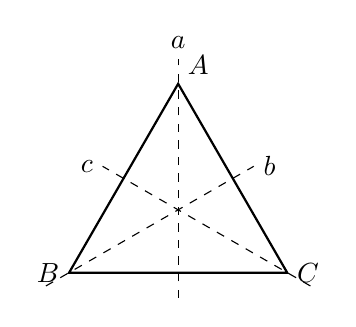
\begin{tikzpicture}[scale=.8]
\coordinate(A)at(0,2);\coordinate(B)at(-1.732,-1);\coordinate(C)at(1.732,-1);
\draw[thick](A)--(B)--(C)--cycle;
\draw[dashed](0,-1.4)--(0,2.4)node[above]{$a$};
\draw[dashed](-2.1,-1.21)--(1.2,.69)node[right]{$b$};
\draw[dashed](2.1,-1.21)--(-1.2,.69)node[left]{$c$};
\node[above right]at(A){$A$};\node[left]at(B){$B$};\node[right]at(C){$C$};
\end{tikzpicture}\end{center}
\end{exercise}
\begin{solution}
官方关系重编，完整表由置换复算。以顶点去向表示每个元素：
$I=(A,B,C)$、$R_+=(C,A,B)$、$R_-=(B,C,A)$、
$R_a=(A,C,B)$、$R_b=(C,B,A)$、$R_c=(B,A,C)$。
例如先反射$a$再顺转，$(A,B,C)\to(A,C,B)\to(C,B,A)$，所以$R_+R_a=R_b$。
\begin{center}\begin{tabular}{c|cccccc}
\toprule
$R_iR_j$&$I$&$R_+$&$R_-$&$R_a$&$R_b$&$R_c$\\\midrule
$I$&$I$&$R_+$&$R_-$&$R_a$&$R_b$&$R_c$\\
$R_+$&$R_+$&$R_-$&$I$&$R_b$&$R_c$&$R_a$\\
$R_-$&$R_-$&$I$&$R_+$&$R_c$&$R_a$&$R_b$\\
$R_a$&$R_a$&$R_c$&$R_b$&$I$&$R_-$&$R_+$\\
$R_b$&$R_b$&$R_a$&$R_c$&$R_+$&$I$&$R_-$\\
$R_c$&$R_c$&$R_b$&$R_a$&$R_-$&$R_+$&$I$\\
\bottomrule\end{tabular}\end{center}

表不关于主对角线对称：$R_aR_+=R_c\ne R_b=R_+R_a$，所以非Abel。恒等元、$R_+R_-=I$及各反射平方$I$可用来核查整张表。
\end{solution}
\originalsection{同位旋的动力学含义}
\begin{exercise}\label{ex:rec-4-2}
Recitation 4题2。比较(a)$p+p\to d+\pi^+$、(b)$p+n\to d+\pi^0$、(c)$n+n\to d+\pi^-$。氘核$I=0$，pion$I=1$，强作用守恒同位旋，截面正比振幅模平方。求$\sigma_a:\sigma_b:\sigma_c$，按相同运动学及忽略电磁修正比较。
\end{exercise}
\begin{solution}
据官方题意独立作Clebsch--Gordan分解；官方答案的截图标为CC排除材料，不复用。取$p=\ket{\frac12,+\frac12}$、$n=\ket{\frac12,-\frac12}$。末态$d\pi$只有$I=1$，而
\begin{equation}
 \ket{pp}=\ket{1,1},\quad \ket{nn}=\ket{1,-1},\quad
 \ket{pn}=\frac1{\sqrt2}\ket{1,0}+\frac1{\sqrt2}\ket{0,0}.
\end{equation}
守恒的强作用只取$pn$中的$I=1$成分。等同位旋约化振幅记$\mathcal A$，三道分别为$\mathcal A,\mathcal A/\sqrt2,\mathcal A$，所以$\sigma_a:\sigma_b:\sigma_c=2:1:2$。
若比较的束能给不同相空间，或保留带电粒子的库仑作用，须再乘对应因子；同位旋比例指的是这些差异剥离后的理想关系。
\end{solution}
\begin{exercise}\label{ex:rec-5-1}
Recitation 5题1。检验Gell-Mann--Nishijima公式对$u,d,s$夸克成立。给$\bar u,\bar d,\bar s$分配同位旋并再检验。原答案记$A$作重子数，本稿用$B$避免与核质量数混淆。
\end{exercise}
\begin{solution}
官方表重编。公式$Q=I_3+(B+S)/2$中$Q$以正元电荷为单位；反夸克的$B,S,I_3,Q$均为对应夸克的相反数。
\begin{center}\begin{tabular}{c|rrrr}\toprule
态&$I_3$&$B$&$S$&$Q$\\\midrule
$u$&$1/2$&$1/3$&$0$&$2/3$\\
$d$&$-1/2$&$1/3$&$0$&$-1/3$\\
$s$&$0$&$1/3$&$-1$&$-1/3$\\
$\bar u$&$-1/2$&$-1/3$&$0$&$-2/3$\\
$\bar d$&$1/2$&$-1/3$&$0$&$1/3$\\
$\bar s$&$0$&$-1/3$&$1$&$1/3$\\\bottomrule
\end{tabular}\end{center}
$u,d$属于$I=1/2$双重态，$s$是该强同位旋SU(2)下的$I=0$态。反双重态的相位约定可能影响基矢写法，但不改变$I_3$和电荷。
\end{solution}
\begin{exercise}\label{ex:rec-5-2}
Recitation 5题2。$\alpha$为两质子两中子的$^4$He核。原题假设没有束缚的$^4$H或$^4$Li，据此推断$\alpha$同位旋；解释题中“$d+d\to\alpha\pi^0$未被观察”的说法。会预期束缚$^4$Be存在吗？原题末句写“four neutrinos”，但官方解答讨论$nnnn$，请分别说明。
\end{exercise}
\begin{solution}
官方同位旋模型重编并补限制。在忽略电磁与同位旋破缺、把所论束缚能级当作同一多重态的近似内，$I\ge1$的$I_3=0$态应有$I_3=\pm1$伙伴；缺少相应束缚伙伴支持$\alpha$基态$I=0$。这不排除别的激发态或不束缚共振，也不能只凭不存在某同位素推断所有核力谱。

两氘初态$I=0$，$\alpha\pi^0$末态$I=1$，所以严格守恒同位旋的强作用振幅为零。源题的“未被观察”不是可沿用的实验事实：2003年已报告该电荷对称破缺反应，见\url{https://doi.org/10.1103/PhysRevLett.91.142302}。小的夸克质量差与电磁效应能给非零振幅；这恰说明选择定则的近似范围。

按官方意图讨论四核子：$pppp$与$nnnn$分别为$I_3=\pm2$，若束缚且具有同一$I=2$强作用多重态，则还须有$^4$H、$^4$He、$^4$Li伙伴。因此源题模型不预期这些四核子束缚态。四中子短寿命共振的报道不等于稳定束缚态，亦不是本简化多重态论证所能排除的对象（Duer等，2022，\url{https://doi.org/10.1038/s41586-022-04827-6}）。若按字面“四中微子”，它们没有核子强同位旋与强核力，本题的核子多重态推理不能用于判断中微子束缚；应先纠正这项源文字错配。
\end{solution}
\originalsection{颜色八重态的基底变换}
\begin{exercise}\label{ex:rec-12-1}
Recitation 12题1。颜色变换$c'=Uc$，$U$为行列式1的幺正矩阵。原件用基底顺序$(r,b,g)$，
\begin{equation}
 U=\begin{pmatrix}0&1&0\\0&0&1\\1&0&0\end{pmatrix},\quad
 \ket3=\frac{r\bar r-b\bar b}{\sqrt2},\quad
 \ket8=\frac{r\bar r+b\bar b-2g\bar g}{\sqrt6}.
\end{equation}
因此$r\to g,g\to b,b\to r$。求$\ket{3'}=\alpha\ket3+\beta\ket8$、$\ket{8'}=\gamma\ket3+\delta\ket8$的四个系数。
\end{exercise}
\begin{solution}
官方$\alpha,\beta$计算重编，另两个系数补全。反颜色按$U^*$变换，这里$U$为实矩阵。直接作用得
$\ket{3'}=(g\bar g-r\bar r)/\sqrt2$、
$\ket{8'}=(g\bar g+r\bar r-2b\bar b)/\sqrt6$。
匹配三个正交颜色对的系数，
\begin{equation}
 \alpha=-\frac12,\quad\beta=-\frac{\sqrt3}2,\quad
 \gamma=\frac{\sqrt3}2,\quad\delta=-\frac12.
\end{equation}
所得二维矩阵正交且三次作用为单位矩阵，与循环$U^3=I$一致。它混合的是同一八重态空间中的两个基矢，并未产生新的独立胶子态；若误改颜色基底顺序，系数符号也会错。
\end{solution}
